\section{Service Water Heating}

Service water heating (SWH) includes all water heating usage other than space heating and process requirements. This includes general water heating for uses such as sink faucets and showers, but also building-type-specific uses like commercial dish washing and laundry. This section describes how SWH equipment, fuel type, and usage is incorporated into ComStock models.   

\subsection{Service Water Heating Fuel Type}
\label{sec:SWH_Fuel_Type}

It would be logical to assume that the SWH system in a building would use the same fuel as the space heating system. An examination of the CBECS 2012 data \citep{eia2012cbecs} shows that this is the most common case, but it is not always true. In particular, it appears that building types that have large SWH loads, such as hotels and hospitals, are much more likely to use natural gas for SWH, regardless of what their space heating fuel is, presumably because of fuel cost differences. In contrast, building types with low SWH loads are more likely to use electricity for SWH, presumably because of the ease and cost of running wiring compared to installing natural gas piping.

To represent this variability, we used the CBECS 2012 data to create a distribution of SWH fuels for each combination of space heating fuel and building type. The resulting distribution of floor area served by various SWH fuels is shown in Figure \ref{fig:swh_fuel_dist}. As described in Section \ref{sec:HVAC_System_Type_Heating_Fuel_Type}, the prevalence of different space heating fuel varies considerably by county. Because the service water heating fuel depends on the space heating fuel, the probabilities at a stock level are heavily skewed toward the more common space heating fuels, as shown in Figure \ref{fig:swh_fuel_area}.

\begin{figure}[ht!]
  \centering
  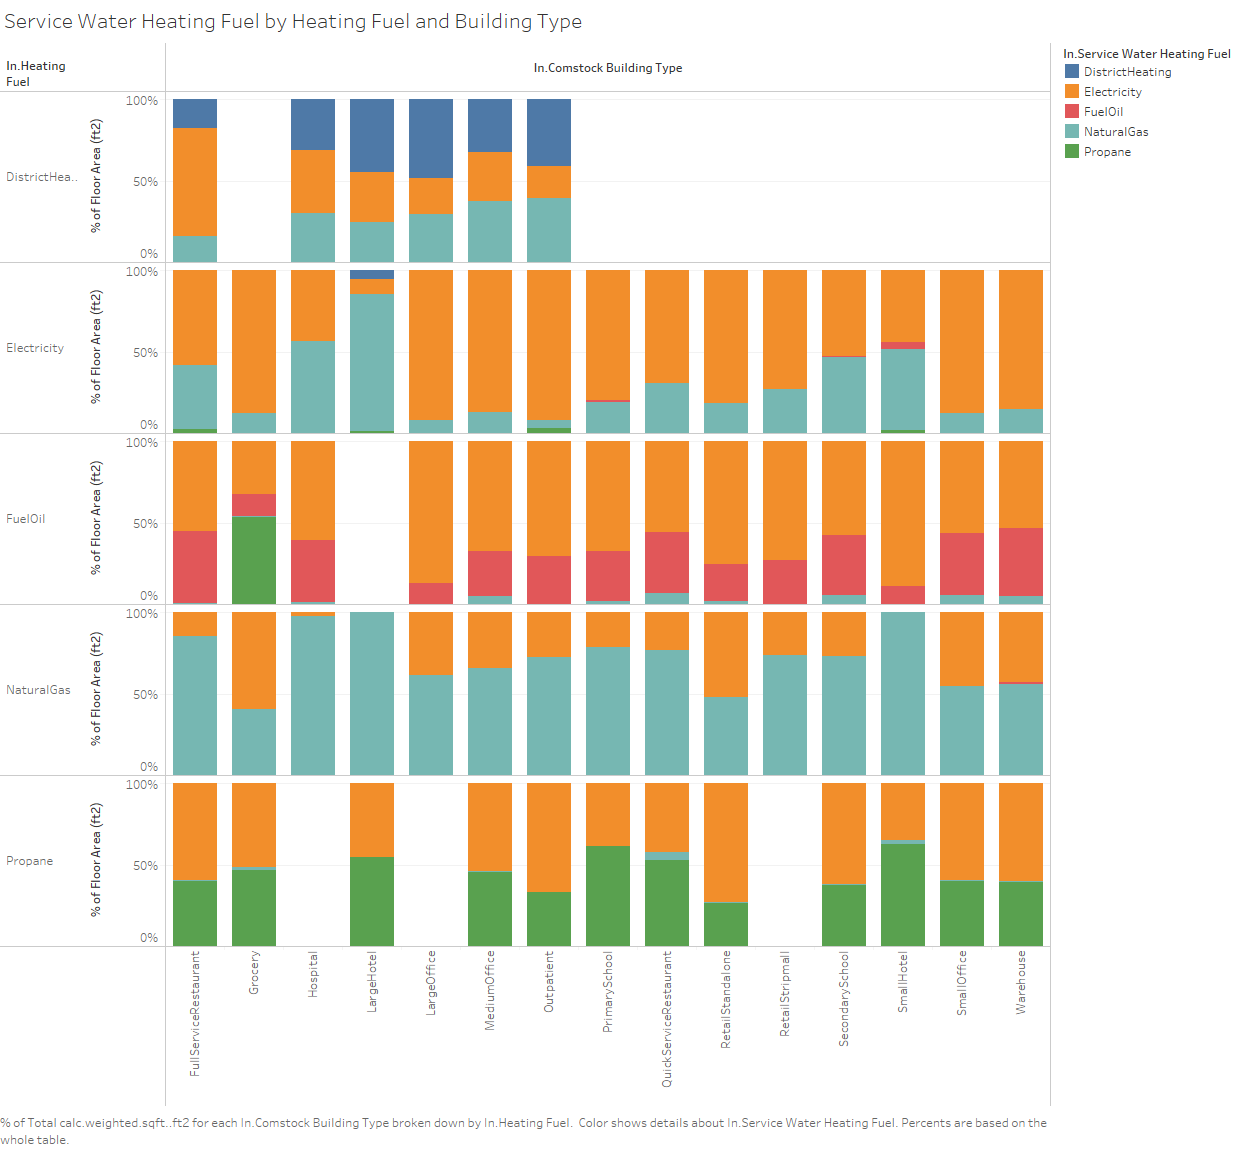
\includegraphics[width=\textwidth]{figures/swh_fuel_dist.png}
  \caption[Distribution of service water heating fuel by space heating fuel and building type]{Area-weighted distribution of service water heating fuel by space heating fuel and building type.}
  \label{fig:swh_fuel_dist}
\end{figure}

\begin{figure}[ht!]
  \centering
  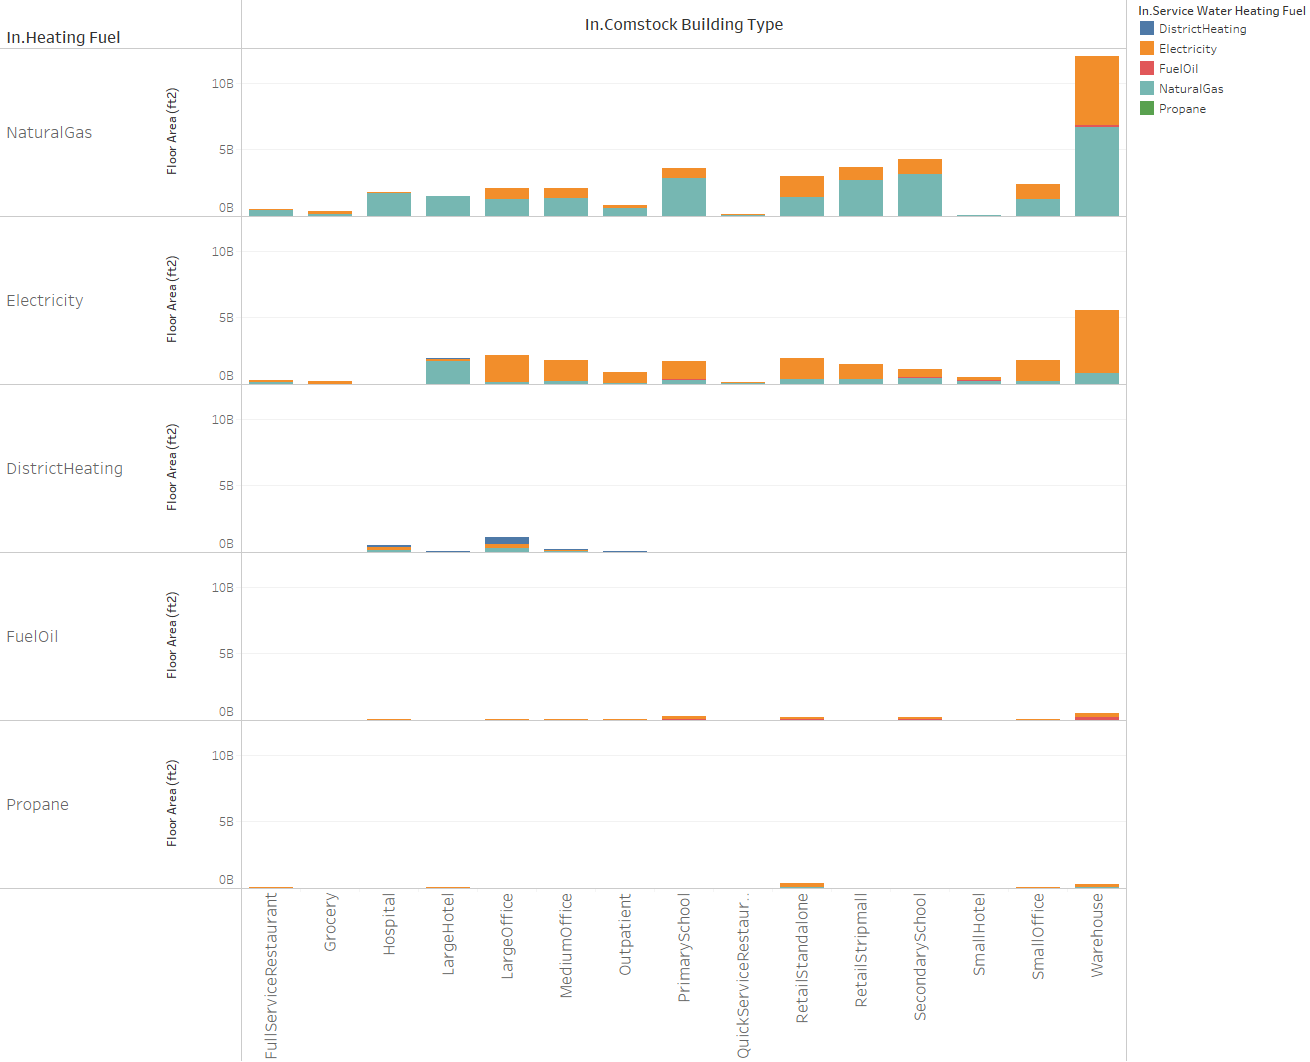
\includegraphics[width=\textwidth]{figures/swh_fuel_area.png}
  \caption[Floor area served by each service water heating fuel by space heating fuel and building type]{Floor area served by each service water heating fuel by space heating fuel and building type.}
  \label{fig:swh_fuel_area}
\end{figure}

\subsection{Service Water Heating System Type}

Service water heaters in ComStock models are all storage tank style, and are either fuel combustion (natural gas, fuel oil, or propane) or electric resistance, as discussed in  Section~\ref{sec:SWH_Fuel_Type}. Service water heaters with district heating as the fuel type receive hot water from off-site; therefore, these models do not include an on-site water heater. ComStock does not currently model instantaneous water heaters or heat pump water heaters. A single water heater is used to meet the demands of the entire building, unless a booster water loop is used, in which case a separate water heater system will be modeled for the boost loop. Booster loops are included for buildings with kitchen space types. These booster water heaters increase the temperature for some portion of the water for uses that need higher temperatures such as dishwashing. See Section~\ref{sec:space_type_ratios} for details on the space type ratios for each building type. In space types with booster water heaters, 60\% of peak flow is assigned to the booster water heater, and the remaining 40\% is assigned to the standard water heater.

The design temperature of standard water heaters in ComStock is 140°F with a 3.6°F deadband temperature difference allowance. Booster water heaters for kitchens have a target temperature of 180°F; this assumption comes from the DOE prototype models to account for dishwashing in kitchens. The ambient air temperature for tank heat loss is assumed to be 72°F. No parasitic losses or part load performance modifiers are included at this time.

%TODO: Discuss heat exchanger for booster water heaters? AP: I don't think this is necessary right now.

\subsection{Service Water Heating Efficiencies}

ComStock water heater efficiencies follow the requirements of ASHRAE-90.1. ComStock currently only models non-condensing units, so water heaters with a combustion fuel source are all roughly 80\% efficient, whereas electric resistance water heaters are roughly 100\% efficient. The efficiency parameters used to calculate the exact water heater efficiencies are summarized in Table~\ref{tab:water_heater_eff} based on SWH template, SWH fuel type, and SWH heater capacity. 

%\begin{table}
\centering
\scriptsize
\caption[Water Heater Efficiency]{Water Heating Efficiency by HVAC Template, Heater Capacity, and Fuel Type}
\label{tab:water_heater_eff}
\begin{tabular}{|p{0.5in}|p{0.5in}|p{0.3in}|p{0.3in}|p{0.3in}|p{0.3in}|p{0.3in}|p{0.3in}|p{0.3in}|p{0.3in}|p{0.3in}|p{0.3in}|p{1in}|}
\hline
\textbf{Template} &
  \textbf{Fuel Type} &
  \textbf{Minimum Capacity (Btu/hr)} &
  \textbf{Maximum Capacity (Btu/hr)} &
  \textbf{Energy Factor Base (\%)} &
  \textbf{Energy Factor Volume Derate (\%/gal)} &
  \textbf{Standby Loss Base (Btu/hr)} &
  \textbf{Standby Loss Capacity Allowance} &
  \textbf{Standby Loss Volume Allowance (Btu/hr*gal)} &
  \textbf{Hourly Loss Base (\%)} &
  \textbf{Hourly Loss Volume Allowance (\%/gal)} &
  \textbf{Thermal Efficiency (\%)} &
  \textbf{Notes} \\ \hline
\multirow{3}{*}{\parbox{0.5in}{\textbf{Pre-1980 Through 1980--2004}}} &
Electricity & 0 & 40945.99 & 0.93 & 0.00132 & & & & & & & \multirow{3}{*}{From DOE Reference Buildings} \\ \cline{2-12} &
Electricity & 40946 & No max & & & 20 & & 35 & & & & \\ \cline{2-12} &
Natural gas & 0 & No max & & & & & & & & 0.78 & \\ \hline
\multirow{4}{*}{\parbox{0.5in}{\textbf{90.1-2004 Through 2010}}} &
Electricity & 0 & 40945.99 & 0.93 & 0.00132 & & & & & & & \multirow{4}{*}{From 90.1 Table 7.8} \\ \cline{2-12} &
Electricity & 40946 & No max & & & 20 & & 35 & & & & \\ \cline{2-12} &
Natural gas & 0 & 74999.99 & 0.62 & 0.0019 & & & & & & & \\ \cline{2-12} &
Natural gas & 75000 & No max & & & & 800 & 110 & & & 0.8 & \\ \hline
\multirow{4}{*}{\textbf{90.1-2013}} &
Electricity & 0 & 40945.99 & 0.97 & 0.00132 & & & & & & & \multirow{4}{*}{From 90.1-2013 Table 7.8} \\ \cline{2-12} &
Electricity & 40946 & No max & & & & & & 0.3 & 27 & & \\ \cline{2-12} &
Natural gas & 0 & 74999.99 & 0.67 & 0.0019 & & & & & & & \\ \cline{2-12} &
Natural gas & 75000 & No max & & & & 800 & 110 & & & 0.8 & \\ \hline
\multirow{4}{*}{\parbox{0.5in}{\textbf{90.1-2016 Through 2019}}} &
Electricity & 0 & 40945.99 & 0.96 & 0.0003 & & & & & & & From 90.1 Table F-2, Rated Storage Volume \textless{}= 55 gal \\ \cline{2-13} &
Electricity & 40946 & No max & & & & & & 0.3 & 27 & & \\ \cline{2-13} &
Natural gas & 0 & 74999.99 & 0.675 & 0.0015 & & & & & & & From 90.1 Table F-2, Rated Storage Volume \textless{}= 55 gal \\ \cline{2-13} &
Natural gas & 75000 & No max & & & & 800 & 110 & & & 0.8 & \\ \hline
\end{tabular}
\end{table}

\subsection{Service Water Heating Usage and Schedules}

SWH usage for a given time step is based on a design peak gal/min flow rate multiplied by a usage fraction schedule. For example, if a given model has a design SWH flow rate of 10 gal/min, and the schedule value for the time step is 0.5, the SWH flow rate for the time step will be 5 gal/min. The flow rate values in ComStock come from the DOE prototype/reference building models, and are summarized in Tables~\ref{tab:swh_flow_rates_p1} through \ref{tab:swh_flow_rates_p3}.

In ComStock, the design flow rates are specified at the space type level. Then, these rates are aggregated to form a building-level design flow rate. The exception to this is SWH loads for kitchens, which are grouped into their own separate water heater system. These design flow rates are then multiplied by the usage fraction schedules, which specify the fraction of the design flow rate drawn for each time step. The usage fraction schedules in ComStock are derived from the DOE prototype/reference Buildings, and are summarized for each building type in Figures~\ref{fig:swh_sched_fsr} through ~\ref{fig:swh_sched_strip_mall}. The default schedule assignments for each space type and vintage are shown in Tables~\ref{tab:swh_flow_rates_p1} through ~\ref{tab:swh_flow_rates_p3}. However, these schedules are modified according to the hours of operation of the building, as described in Section~\ref{sec:hoo}. 

%TODO: Describe where flow rates and schedules come from
%TODO: Describe water heater tank and capacity sizing methods
%TODO: Describe the HX things for booster water heaters.

%\begin{table}
\centering
\small
\caption[Service Water Heating Flow Rate and Schedules Part 1]{Service Water Heating Flow Rate and Schedule Assignments Based on Template, Building Type, and Space Type (Part 1 of 3)}
\label{tab:swh_flow_rates_p1}
\begin{tabular}{|p{3cm}|p{3cm}|p{3cm}|p{3cm}|p{3cm}|}
\hline
\textbf{Template} &
  \textbf{Building Type} &
  \textbf{Space Type} &
  \textbf{Service Water   Heating Peak Flow per Area (gal/h*ft$^2$)} &
  \textbf{Service Water   Heating Schedule} \\ \hline
\textbf{All}                     & FullServiceRestaurant & Kitchen     & 0.08861 & RestaurantSitDown   BLDG\_SWH\_SCH           \\ \hline
\textbf{All}                     & Hospital              & ER\_Exam    & 0.00333 & Hospital   BLDG\_SWH\_EXTD\_SCH              \\ \hline
\textbf{All}                     & Hospital              & ER\_Trauma  & 0.00333 & Hospital   BLDG\_SWH\_EXTD\_SCH              \\ \hline
\textbf{All}                     & Hospital              & ER\_Triage  & 0.00333 & Hospital   BLDG\_SWH\_EXTD\_SCH              \\ \hline
\textbf{All}                     & Hospital              & Kitchen     & 0.015   & Hospital   BLDG\_SWH\_EXTD\_SCH              \\ \hline
\textbf{All}                     & Hospital              & Lab         & 0.0007  & Hospital BLDG\_SWH\_SCH                      \\ \hline
\textbf{All}                     & Hospital              & OR          & 0.00333 & Hospital BLDG\_SWH\_SCH                      \\ \hline
\textbf{All}                     & Hospital              & PatRoom     & 0.00357 & Hospital   BLDG\_SWH\_EXTD\_SCH              \\ \hline
\textbf{All}                     & Hospital              & PhysTherapy & 0.00019 & Hospital BLDG\_SWH\_SCH                      \\ \hline
\textbf{All}                     & Hospital              & Radiology   & 0.00019 & Hospital   BLDG\_SWH\_EXTD\_SCH              \\ \hline
\textbf{All}                     & LargeHotel            & GuestRoom   & 0.00298 & HotelLarge   GuestRoom\_SWH\_Sch             \\ \hline
\textbf{All}                     & LargeHotel            & GuestRoom2  & 0.00473 & HotelLarge   GuestRoom\_SWH\_Sch             \\ \hline
\textbf{All}                     & LargeHotel            & GuestRoom2  & 0.08994 & HotelLarge   GuestRoom\_SWH\_Sch             \\ \hline
\textbf{All}                     & LargeHotel            & GuestRoom3  & 0.00298 & HotelLarge   GuestRoom\_SWH\_Sch             \\ \hline
\textbf{All}                     & LargeHotel            & GuestRoom4  & 0.00473 & HotelLarge   GuestRoom\_SWH\_Sch             \\ \hline
\textbf{All}                     & LargeHotel            & GuestRoom4  & 0.0426  & HotelLarge   GuestRoom\_SWH\_Sch             \\ \hline
\textbf{All}                     & LargeHotel            & GuestRoom5  & 0.0036  & HotelLarge   GuestRoom\_SWH\_Sch             \\ \hline
\textbf{All}                     & LargeHotel            & GuestRoom6  & 0.00294 & HotelLarge   GuestRoom\_SWH\_Sch             \\ \hline
\textbf{All}                     & LargeHotel            & GuestRoom7  & 0.00215 & HotelLarge   GuestRoom\_SWH\_Sch             \\ \hline
\textbf{All}                     & LargeHotel            & GuestRoom8  & 0.00473 & HotelLarge   GuestRoom\_SWH\_Sch             \\ \hline
\textbf{All}                     & LargeHotel            & Kitchen     & 0.1196  & HotelLarge   BLDG\_SWH\_SCH                  \\ \hline
\textbf{90.1-2004 and Later} & LargeHotel            & Laundry     & 0.18643 & HotelLarge   LaundryRoom\_SWH\_Sch\_Post2004 \\ \hline
\textbf{Pre 90.1-2004}  & LargeHotel            & Laundry     & 0.18643 & HotelLarge   LaundryRoom\_SWH\_Sch\_Pre2004  \\ \hline
\end{tabular}
\end{table}
%\begin{table}
\centering
\small
\caption[Service Water Heating Flow Rate and Schedules Part 2]{Service Water Heating Flow Rate and Schedule Assignments Based on Template, Building Type, and Space Type (Part 2 of 3)}
\label{tab:swh_flow_rates_p2}
\begin{tabular}{|p{3cm}|p{3cm}|p{3cm}|p{3cm}|p{3cm}|}
\hline
\textbf{Template} &
  \textbf{Building Type} &
  \textbf{Space Type} &
  \textbf{Service Water   Heating Peak Flow per Area (gal/h*ft$^2$)} &
  \textbf{Service Water   Heating Schedule} \\ \hline
\textbf{Pre 90.1-2004}  & Office          & MediumOffice -   Elec/MechRoom       & 0.01845 & Medium Office Bldg   Swh           \\ \hline
\textbf{90.1-2004 and Later} & Office          & MediumOffice -   Elec/MechRoom       & 0.03171 & OfficeMedium   BLDG\_SWH\_SCH      \\ \hline
\textbf{All}                     & Office          & Restroom                             & 0.20471 & OfficeLarge   BLDG\_SWH\_SCH       \\ \hline
\textbf{All}                     & Office          & SmallOffice -   Elec/MechRoom        & 0.00055 & OfficeSmall   BLDG\_SWH\_SCH       \\ \hline
\textbf{Pre 90.1-2004}  & Office          & WholeBuilding - Lg   Office          & 0.00013 & OfficeLarge   BLDG\_SWH\_SCH       \\ \hline
\textbf{90.1-2004 and Later} & Office          & WholeBuilding - Lg   Office          & 0.00052 & OfficeLarge   BLDG\_SWH\_SCH       \\ \hline
\textbf{All}                     & Office          & WholeBuilding - Lg   Office-basement & 0.00052 & OfficeLarge   BLDG\_SWH\_SCH       \\ \hline
\textbf{All}                     & Office          & WholeBuilding - Lg   Office-others   & 0.00052 & OfficeLarge   BLDG\_SWH\_SCH       \\ \hline
\textbf{Pre 90.1-2004}  & Office          & WholeBuilding - Md   Office          & 0.00055 & OfficeMedium   BLDG\_SWH\_SCH      \\ \hline
\textbf{90.1-2004 and Later} & Office          & WholeBuilding - Md   Office          & 0.00095 & OfficeMedium   BLDG\_SWH\_SCH      \\ \hline
\textbf{All}                     & Office          & WholeBuilding - Sm   Office          & 0.00055 & OfficeSmall   BLDG\_SWH\_SCH       \\ \hline
\textbf{All}                     & Retail          & Back\_Space                          & 0.00535 & RetailStandalone   BLDG\_SWH\_SCH  \\ \hline
\textbf{All}                     & SecondarySchool & Gym                                  & 0.0075  & SchoolSecondary   BLDG\_SWH\_SCH   \\ \hline
\textbf{All}                     & SecondarySchool & Gym - audience                       & 0.0075  & SchoolSecondary   BLDG\_SWH\_SCH   \\ \hline
\textbf{All}                     & SecondarySchool & Kitchen                              & 0.0572  & SchoolSecondary   BLDG\_SWH\_SCH   \\ \hline
\textbf{All}                     & SecondarySchool & Restroom                             & 0.0231  & SchoolSecondary   BLDG\_SWH\_SCH   \\ \hline
\textbf{All}                     & SmallHotel      & GuestRoom                            & 0.00499 & HotelSmall   GuestRoom\_SHW\_Sch   \\ \hline
\textbf{Pre 90.1-2004}  & SmallHotel      & GuestRoom123Occ                      & 0.00499 & HotelSmall   GuestRoom\_SHW\_Sch   \\ \hline
\textbf{90.1-2004 and Later} & SmallHotel      & GuestRoom123Occ                      & 0.00632 & HotelSmall   GuestRoom\_SHW\_Sch   \\ \hline
\textbf{Pre 90.1-2004}  & SmallHotel      & GuestRoom123Vac                      & 0.00499 & HotelSmall   GuestRoom\_SHW\_Sch   \\ \hline
\textbf{90.1-2004 and Later} & SmallHotel      & GuestRoom123Vac                      & 0.00632 & HotelSmall AlwaysOff               \\ \hline
\textbf{Pre 90.1-2004}  & SmallHotel      & GuestRoom4Occ                        & 0.00499 & HotelSmall   GuestRoom\_SHW\_Sch   \\ \hline
\textbf{90.1-2004 and Later} & SmallHotel      & GuestRoom4Occ                        & 0.00632 & HotelSmall   GuestRoom\_SHW\_Sch   \\ \hline
\textbf{Pre 90.1-2004}  & SmallHotel      & GuestRoom4Vac                        & 0.00499 & HotelSmall   GuestRoom\_SHW\_Sch   \\ \hline
\textbf{90.1-2004 and Later} & SmallHotel      & GuestRoom4Vac                        & 0.00632 & HotelSmall AlwaysOff               \\ \hline
\textbf{All}                     & SmallHotel      & Laundry                              & 0.0641  & HotelSmall   LaundryRoom\_SHW\_Sch \\ \hline
\end{tabular}
\end{table}
%\begin{table}
\centering
\small
\caption[Service Water Heating Flow Rate and Schedules Part 3]{Service Water Heating Flow Rate and Schedule Assignments Based on Template, Building Type, and Space Type (part 3 of 3)}
\label{tab:swh_flow_rates_p3}
\begin{tabular}{|p{3cm}|p{3cm}|p{3cm}|p{3cm}|p{3cm}|}
\hline
\textbf{Template} &
  \textbf{Building Type} &
  \textbf{Space Type} &
  \textbf{Service Water   Heating Peak Flow per Area (gal/h*ft$^2$)} &
  \textbf{Service Water   Heating Schedule} \\ \hline
\textbf{Pre 90.1-2004}  & Outpatient             & Anesthesia      & 0.00926 & OutPatientHealthCare   BLDG\_SWH\_SCH\_Pre2004 \\ \hline
\textbf{90.1-2004 and Later} & Outpatient             & Anesthesia      & 0.01852 & OutPatientHealthCare   BLDG\_SWH\_SCH          \\ \hline
\textbf{Pre 90.1-2004}  & Outpatient             & MRI             & 0.00227 & OutPatientHealthCare   BLDG\_SWH\_SCH\_Pre2004 \\ \hline
\textbf{90.1-2004 and Later} & Outpatient             & MRI             & 0.00455 & OutPatientHealthCare   BLDG\_SWH\_SCH          \\ \hline
\textbf{Pre 90.1-2004}  & Outpatient             & MRI\_Control    & 0.00595 & OutPatientHealthCare   BLDG\_SWH\_SCH\_Pre2004 \\ \hline
\textbf{90.1-2004 and Later} & Outpatient             & MRI\_Control    & 0.0119  & OutPatientHealthCare   BLDG\_SWH\_SCH          \\ \hline
\textbf{Pre 90.1-2004}  & Outpatient             & OR              & 0.01271 & OutPatientHealthCare   BLDG\_SWH\_SCH\_Pre2004 \\ \hline
\textbf{90.1-2004 and Later} & Outpatient             & OR              & 0.02542 & OutPatientHealthCare   BLDG\_SWH\_SCH          \\ \hline
\textbf{Pre 90.1-2004}  & Outpatient             & PACU            & 0.00316 & OutPatientHealthCare   BLDG\_SWH\_SCH\_Pre2004 \\ \hline
\textbf{90.1-2004 and Later} & Outpatient             & PACU            & 0.00633 & OutPatientHealthCare   BLDG\_SWH\_SCH          \\ \hline
\textbf{Pre 90.1-2004}  & Outpatient             & PhysicalTherapy & 0.00106 & OutPatientHealthCare   BLDG\_SWH\_SCH\_Pre2004 \\ \hline
\textbf{90.1-2004 and Later} & Outpatient             & PhysicalTherapy & 0.00211 & OutPatientHealthCare   BLDG\_SWH\_SCH          \\ \hline
\textbf{Pre 90.1-2004}  & Outpatient             & PreOp           & 0.0038  & OutPatientHealthCare   BLDG\_SWH\_SCH\_Pre2004 \\ \hline
\textbf{90.1-2004 and Later} & Outpatient             & PreOp           & 0.00759 & OutPatientHealthCare   BLDG\_SWH\_SCH          \\ \hline
\textbf{Pre 90.1-2004}  & Outpatient             & ProcedureRoom   & 0.00351 & OutPatientHealthCare   BLDG\_SWH\_SCH\_Pre2004 \\ \hline
\textbf{90.1-2004 and Later} & Outpatient             & ProcedureRoom   & 0.00702 & OutPatientHealthCare   BLDG\_SWH\_SCH          \\ \hline
\textbf{Pre 90.1-2004}  & Outpatient             & Xray            & 0.00111 & OutPatientHealthCare   BLDG\_SWH\_SCH\_Pre2004 \\ \hline
\textbf{90.1-2004 and Later} & Outpatient             & Xray            & 0.00222 & OutPatientHealthCare   BLDG\_SWH\_SCH          \\ \hline
\textbf{All}                     & PrimarySchool          & Kitchen         & 0.05531 & SchoolPrimary   BLDG\_SWH\_SCH                 \\ \hline
\textbf{All}                     & PrimarySchool          & Restroom        & 0.02763 & SchoolPrimary   BLDG\_SWH\_SCH                 \\ \hline
\textbf{Pre 90.1-2004}  & QuickServiceRestaurant & Kitchen         & 0.032   & QuickServiceRestaurant   Bldg Swh              \\ \hline
\textbf{90.1-2004 and Later} & QuickServiceRestaurant & Kitchen         & 0.032   & RestaurantFastFood   BLDG\_SWH\_SCH            \\ \hline
\end{tabular}
\end{table}





